\section{VCO: Voltage Controlled Oscillator}
Esta secci\'on se propone el dise\~no de un oscilador de se\~nales senoidales cuya frecuencia pueda ser controlada por una tensi\'on de entrada,
de forma tal que para un dado rango de tensiones, se pueda producir la se\~nal deseada que var\'ie en un rango esperado de frecuencias.
En la Fig. \ref{fig:esquema_general_ejercicio_3} se ilustra un esquema general del sistema deseado.

\begin{figure}[H]
    \centering
    \includegraphics[scale=0.5]{../EJ3/Recursos/system_scheme.png}
    \caption{Esquema general del sistema propuesto}
    \label{fig:esquema_general_ejercicio_3}
\end{figure}


\subsection{Introducci\'on te\'orica}
El objetivo de esta introducci\'on es establecer las bases te\'oricas sobre las cuales se construye
el an\'alisis desarrollado para el dise\~no del sistema propuesto. No obstante, se asume que el lector posee
una base te\'orica sobre algunos conceptos, lo cual se ir\'a indicando a lo largo de tal an\'alisis.

\subsubsection{Distorsi\'on Arm\'onica}
La teor\'ia de series generalizadas de Fourier establece que cualquier se\~nal peri\'odica, es decir una funci\'on dada tal que
$f: I\!R -> I\!R$ que cumple tener un per\'iodo fundamental dado $f(t + T) = f(t)$, con T perteneciente a los reales positivos, puede
ser proyectada sobre un espacio vectorial descripto por su base ortonormal.
En otras palabras, la serie trigonométrica de Fourier como caso particular permite describir un se\~nal peri\'odica como combinaci\'on 
lineal de funciones seno y coseno. Se suele denominar a cada una de estas componentes como arm\'onicos cuyas frecuencias son m\'ultiplos de la 
frecuencia fundamental, y desde un punto de vista espectral es sencillo observar la distribuci\'on de potencia de la se\~nal para cada frecuencia
arm\'onica.

\begin{figure}[H]
    \centering
    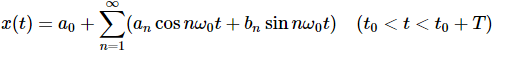
\includegraphics[scale=0.6]{../EJ3/Recursos/fourier_series.PNG}
    \caption{Series de Fourier}
\end{figure}


\begin{figure}[H]
    \centering
    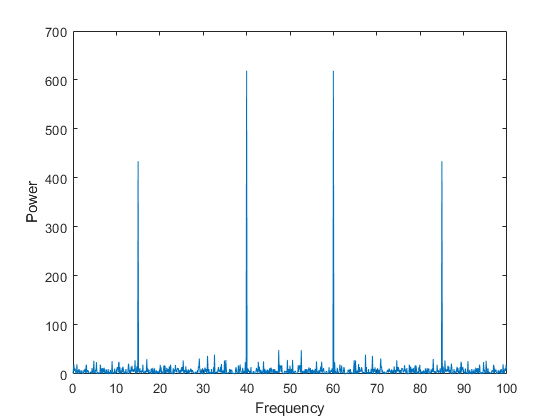
\includegraphics[scale=0.4]{../EJ3/Recursos/BasicSpectralAnalysisExample_01.png} 
    \caption{Espectro en frecuencia}
\end{figure}

La distorsi\'on arm\'onica puede ser entendida como la presencia de arm\'onicos no deseados que en el dominio temporal alteran o distorsionan la forma
de onda esperada, esto puede pasar como consecuencia del uso de sistemas no lineales o por el l\'imite f\'isico de ancho de banda que suelen tener
los circuitos, aunque no siempre se vuelve apreciable su efecto sobre la eliminaci\'on de los arm\'onicos deseados.
As\'i, una se\~nal senoidal pura \'unicamente contiene su arm\'onico fundamental, y en t\'erminos del espectro en frecuencia s\'olo una componente. Esto permite
estudiar la distorsi\'on de tales se\~nales analizando aquellos componentes arm\'onicos no deseados que pueden aparecen, y se utiliza la expresi\'on de la Ec. \ref{eq:distorsion_de_armonico}
para cuantificarla. La distorsi\'on total se define como se observa en la Ec. \ref{eq:total_distorsion}.

\begin{equation}
    HD_n = \frac{armonico_n}{armonico_{fundamental}}
    \label{eq:distorsion_de_armonico}
\end{equation}

\begin{equation}
    THD = \sqrt{\sum_{n} (HD_n)^{2}}
    \label{eq:total_distorsion}
\end{equation}

\subsubsection{Jitter}
Se define el Jitter como la desviaci\'on pr\'actica del per\'iodo de una se\~nal respecto de su valor te\'orico esperado. Este es un aspecto
a tener en cuenta en el dise\~no y an\'alisis de osciladores, y puede clasificarse generalmente seg\'un si es aleatorio o determin\'istico.

\begin{figure}[H]
    \centering
    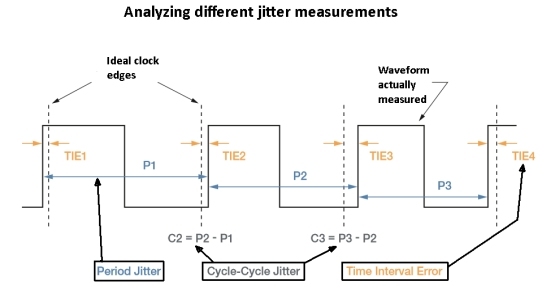
\includegraphics[scale=0.5]{../EJ3/Recursos/different-jitter-measurements.jpg}
    \caption{Diagrama del Jitter medido en un per\'iodo o entre ciclos}
    \label{fig:jitter_diagram}
\end{figure}

El jitter aleatorio corresponde a la desviaci\'on del per\'iodo provocada por el ruido t\'ermico que generan los componentes resistivos en la pr\'actica.
Por otro lado, el jitter determin\'istico consiste en analizar las posibles desviaciones temporales, ya sea de un per\'iodo respecto del valor real, as\'i
como entre per\'iodos de ciclos consecutivos. Esto puede observarse en la Fig. \ref{fig:jitter_diagram}.

\subsection{An\'alisis de circuitos}
Se busca realizar un an\'alisis de los circuitos empleados posteriormente en el dise\~no para facilitar, no s\'olo este proceso,
sino la divisi\'on en etapas seg\'un lo requiera el sistema, teniendo en cuenta las fortalezas y debilidades de cada una de ellas.

\subsubsection{Acondicionamiento lineal de se\~nal}
En la pr\'actica suele ser necesario realizar un acondicionamiento lineal de una se\~nal de entrada, esto implica matem\'aticamente aplicar un desplazamiento
y un escalaje sobre la magnitud de entrada, adaptando el rango de valores de entrada a un rango aceptable de salida. Se propone como circuito para realizar esta transformaci\'on
de las magnitudes, el ilustrado en la Fig. \ref{fig:circuito_acondicionamiento_lineal}.

\begin{figure}[H]
    \centering
    \includegraphics[scale=0.55]{../EJ3/Recursos/circuito_acondicionamiento_lineal.png}
    \caption{Acondicionamiento lineal de se\~nales}
    \label{fig:circuito_acondicionamiento_lineal}
\end{figure}

Se plantean las siguientes ecuaciones, donde se define la salida del amplificador operacional configurado como buffer o seguidor de tensi\'on $V_{OFF}$.

\begin{align*}
    & V_{OFF} = \frac{V_{CC} \cdot R_2}{R_1 + R_2} \\
    & V_o = V_i \cdot \frac{R_4}{R_3 + R_4} \cdot \frac{R_5 + R_6}{R_5}
    + V_{OFF} \cdot \frac{R_3}{R_3 + R_4} \cdot \frac{R_5 + R_6}{R_5}
\end{align*}

Aplicando como criterio para simplificar el manejo algebraico, resulta pr\'actico establecer que se cumpla la condici\'on
$R_3 = R_5$ y $R_4 = R_6$.

\begin{equation}
    V_o = V_i \cdot \frac{R_4}{R_5} + V_{OFF}
\end{equation}

En conclusi\'on, este circuito con esta \'ultima expresi\'on permite de manera sencilla realizar una transformaci\'on que permita adaptar o acondicionar
la se\~nal entrante, conociendo la pendiente y ordenada al origen que se desean como salida. Es importante mencionar que el circuito no garantiza un l\'imite de tensi\'on 
que no sea el de saturaci\'on de los amplificadores, con lo cual a menos que se haga uso de este, ser\'a necesario un circuito limitador de tensi\'on en la salida seg\'un el caso.

\subsubsection{Comparador Schmitt Trigger inversor}
% Explicar el Schmitt Trigger y sus cuentas

\subsubsection{Voltage Controlled Oscillator}
% Explicar el VCO y sus cuentas

\subsubsection{Conversor triangular a senoidal}
% Explicación del circuito!!

\subsection{Dise\~no de VCO}

\subsubsection{Especificaciones y etapas}

\subsubsection{C\'alculo de componentes}

\subsubsection{Simulaci\'on y verificaci\'on}

\subsection{Resultados}

\subsubsection{Mediciones}

\subsubsection{An\'alisis de resultados}

\subsection{Conclusiones}